\documentclass[12pt,a4paper]{article}

\usepackage[utf8]{inputenc}
\usepackage[T1]{fontenc}
\usepackage{lmodern}
\usepackage[margin=1in]{geometry}
\usepackage{amsmath,amssymb}
\usepackage{booktabs}
\usepackage{graphicx}
\usepackage{float}
\usepackage{hyperref}
\usepackage{natbib}
\usepackage{setspace}
\usepackage{threeparttable}

\onehalfspacing

\title{COVID-19 and the Formality Recovery Path in Peru:\\
A Worker-Level Panel DiD Using Sectoral Teleworkability}

\author{
  Research Pipeline Output\\
  \textit{ENAHO Panel Analysis}
}
\date{\today}

\begin{document}

\maketitle

\begin{abstract}
We examine the effect of COVID-19 on labor informality in Peru using a difference-in-differences design that exploits differential occupational exposure via the \citet{dingel2020} teleworkability index. Using five waves of the ENAHO employment panel (2020--2024, 262,733 observations), our continuous treatment specification finds that a one-unit increase in teleworkability is associated with a 19--22 pp smaller informality increase ($p < 0.05$ in 2022 and 2024; $p < 0.10$ in all post-2020 years). The binary specification yields a differential of approximately 9 pp for contact-intensive workers, though this is not statistically significant at the 5\% level with ISCO-clustered standard errors ($p = 0.153$). The differential showed zero attenuation through 2024 (Wald test $p = 0.937$). Survey weights are winsorized and standard errors are clustered at the ISCO-08 2-digit occupation level (40 clusters). The teleworkability index is pre-determined and panel attrition is not differential by treatment ($p = 0.163$). The effect is concentrated in the loss of employer-provided social security rather than firm-size changes. A key limitation is the absence of pre-2020 data to test parallel trends.

\medskip
\noindent \textbf{Keywords:} COVID-19, informality, scarring, difference-in-differences, teleworkability, Peru

\noindent \textbf{JEL Codes:} J46, O17, J21, I18
\end{abstract}

\newpage
\tableofcontents
\newpage

\section{Introduction}
\label{sec:introduction}

Peru's labor market informality rate exceeds 70\%, one of the highest in Latin America. The COVID-19 pandemic, which triggered strict lockdowns and mobility restrictions beginning in March 2020, disrupted formal employment relationships across all sectors---but its impact was not uniform. Workers in contact-intensive occupations, where physical presence is essential and remote work is infeasible, faced the most severe labor disruptions. This paper examines whether these differentially exposed workers experienced a persistent increase in informality or whether they recovered to pre-pandemic formality levels by 2024.

We exploit differential sectoral exposure to COVID-19 mobility restrictions using the \citet{dingel2020} teleworkability index as a source of identifying variation. The index, originally constructed from O*NET task descriptions for U.S. occupations, measures the feasibility of performing each occupation remotely. We map this index to Peruvian occupation codes (ISCO-08) via a crosswalk, creating a continuous, pre-determined treatment intensity variable.

Using the ENAHO rotating panel from 2020 to 2024 (Module 500, Employment), we estimate a difference-in-differences specification interacting year dummies with the continuous teleworkability score. Our main specification yields negative interaction coefficients of $-0.19$ to $-0.22$ ($p < 0.05$ in 2022 and 2024), indicating that a one-unit increase in teleworkability is associated with a 19--22 pp smaller informality increase. The binary specification (contact-intensive vs.\ teleworkable) yields a differential of approximately 9 pp, though this is not statistically significant at the 5\% level with ISCO-clustered standard errors ($p = 0.153$ in 2021). The differential persisted unchanged through 2024 (Wald test $p = 0.937$), indicating that the population-level informality gap between occupational groups has not closed over four years.

We emphasize three important caveats. First, our panel begins in 2020---the year of the shock---so we cannot test parallel pre-trends. The identifying assumption of common trends rests on plausibility, not statistical evidence. Second, ENAHO's rotating panel design limits within-individual tracking to approximately two consecutive years. Third, attrition from the panel is not differential by treatment status ($p = 0.163$), but the overall attrition rate is high (78.7\% by 2021).

These findings contribute to the literature on labor market scarring \citep{arulampalam2001} and informality dynamics in developing countries \citep{bosch2025}. The paper proceeds as follows: Section~\ref{sec:literature} reviews the literature, Section~\ref{sec:data} describes the data, Section~\ref{sec:strategy} presents the identification strategy, Section~\ref{sec:results} reports results, Section~\ref{sec:robustness} discusses robustness, and Section~\ref{sec:conclusion} concludes.

\section{Literature Review}
\label{sec:literature}

This paper connects three strands of the literature: labor market scarring, informality in developing countries, and the differential impacts of COVID-19 by occupation.

\subsection{Labor Market Scarring}

The scarring hypothesis holds that adverse labor market shocks can produce persistent effects on workers' employment quality, wages, and formality status long after the initial shock dissipates. \citet{arulampalam2001} document that unemployment spells in the UK carry a wage penalty of 6\% that persists for over a decade. In developing countries, \citet{cruces2012} show that exposure to economic crises in Argentina durably reduced formal sector attachment. The mechanism is that workers displaced into informality face barriers to re-entry---skill depreciation, loss of employer networks, and stigma---creating a ``trap'' that outlasts the shock.

\subsection{Informality in Peru}

Peru has one of the highest informality rates in Latin America, with over 70\% of workers lacking formal employment relationships. \citet{bosch2025} study the effect of enforcement letters on firm formalization, finding modest but significant effects on social security enrollment among large firms. However, the worker-side experience of informality transitions remains underexplored. The COVID-19 pandemic provides a quasi-natural experiment: the lockdowns forced millions of formal workers into informal arrangements, creating a large cohort of ``involuntary informals'' whose subsequent trajectory can be tracked.

\subsection{COVID-19 and Occupation-Based Exposure}

\citet{dingel2020} introduced the teleworkability index, classifying occupations by the feasibility of remote work based on O*NET task descriptions. This index has been widely used as a source of identifying variation for COVID-19's differential labor market impacts. \citet{saltiel2020} adapted the index for developing countries, finding that only 13\% of workers in low- and middle-income countries can work from home, compared to 37\% in the U.S. For Peru specifically, our data shows that 74.6\% of employed workers are in contact-intensive occupations (teleworkability score $< 0.20$), making the country an important setting for studying the long-run consequences of occupation-based COVID exposure.

\section{Data}
\label{sec:data}

\subsection{Data Source}

We use the Encuesta Nacional de Hogares (ENAHO) Module 500 (Employment), Peru's primary household labor force survey conducted by INEI. Our panel covers 2020--2024, with 348,505 individuals and 7,337 variables in wide format. The data is reshaped to long format, yielding 1,742,525 individual-year observations.

\subsection{Sample}

We restrict to working-age (15--65) employed individuals (\texttt{ocu500} = 1), yielding 262,733 observations across 214,413 unique individuals. ENAHO uses a rotating panel design where households are tracked for approximately two consecutive years before replacement; only 0.5\% of individuals are observed in all five waves.

\subsection{Outcome: Informality}

Our primary informality measure is the absence of social security coverage (\texttt{p511a} = 7, ``no insurance through employer''). This captures 19.5\% of employed workers in 2020, rising sharply to 34.5\% in 2021 and stabilizing around 34\% through 2024. We construct two alternative measures for robustness: (i) absence of a written contract (\texttt{p517} $\in \{5, 6\}$) and (ii) employment in a small firm with fewer than 5 workers (\texttt{p510} $\in \{1, 2\}$).

\subsection{Treatment: Teleworkability}

We measure treatment intensity using the \citet{dingel2020} teleworkability index, mapped to ENAHO via a crosswalk from BLS SOC codes to ISCO-08 2-digit occupation codes. The crosswalk aggregates D\&N's 764 occupation-level teleworkability scores to 43 ISCO-08 sub-major groups, then merges with ENAHO's \texttt{p505r4} occupation variable (which follows the ISCO-08 classification). The match rate is 100\% for employed workers.

Our primary treatment measure is the \textit{continuous} teleworkability score (0--1). As a secondary specification, we define a binary indicator: \textbf{contact-intensive} = teleworkability score $< 0.20$. This captures 74.6\% of the employed sample, reflecting Peru's concentration of workers in occupations requiring physical presence (agriculture, construction, personal services, manufacturing). Only 8.2\% of workers are in highly teleworkable occupations (score $\geq 0.50$).

Table~\ref{tab:descriptive} compares contact-intensive and teleworkable workers. Contact-intensive workers have higher baseline informality rates and lower incomes, consistent with the well-documented correlation between occupation type and labor formality in Peru.

\begin{table}[htbp]
\centering
\caption{Descriptive Statistics by Teleworkability}
\label{tab:descriptive}
\begin{tabular}{lccccc}
\toprule
 & \multicolumn{2}{c}{Contact-Intensive} & \multicolumn{2}{c}{Teleworkable} & \\
\cmidrule(lr){2-3} \cmidrule(lr){4-5}
Variable & Mean & N & Mean & N & Diff \\
\midrule
Informality rate & 0.358 & 196,069 & 0.192 & 66,664 & 0.166 \\
Age & 40 & 196,069 & 40 & 66,664 & 0.570 \\
Female & 0.416 & 196,069 & 0.610 & 66,664 & -0.194 \\
Rural & 0.442 & 196,069 & 0.123 & 66,664 & 0.319 \\
Monthly income (soles) & 15440 & 78,180 & 25408 & 38,777 & -9968 \\
\bottomrule
\end{tabular}
\begin{tablenotes}\small
\item Notes: Contact-intensive = teleworkability score $<$ 0.20. Teleworkable = score $\geq$ 0.20. Working-age employed sample (15--65), 2020--2024.
\end{tablenotes}
\end{table}


\subsection{Survey Design}

All estimates use ENAHO's survey expansion factor (\texttt{facpob07}) as sampling weights. Standard errors are clustered at the ISCO-08 2-digit occupation level (40 clusters), the level at which treatment is assigned. We discuss the implications of the rotating panel design for within-individual estimation in Section~\ref{sec:robustness}.

\section{Empirical Strategy}
\label{sec:strategy}

\subsection{Identification}

We exploit the differential exposure of occupations to COVID-19 mobility restrictions using the \citet{dingel2020} teleworkability index as treatment intensity. The identifying assumption is that, absent the pandemic, informality trends would have evolved similarly for contact-intensive and teleworkable workers (parallel trends). Workers in low-teleworkability occupations could not shift to remote work during lockdowns and therefore faced greater disruption to their formal employment relationships.

The teleworkability index is pre-determined: it is constructed from O*NET task descriptions measured before the pandemic and reflects the physical characteristics of occupations, not workers' choices during COVID-19. This mitigates concerns about endogenous treatment assignment.

\subsection{Main Specification}

Our primary specification uses the \textit{continuous} teleworkability score as treatment intensity, avoiding the arbitrary binary classification that places 74.6\% of workers in the ``treated'' group:
\begin{equation}
    \text{Informal}_{it} = \alpha + \sum_{k \neq 2020} \beta_k \cdot D_k + \sum_{k \neq 2020} \gamma_k \cdot (D_k \times \text{TW}_i) + \delta \cdot \text{TW}_i + \varepsilon_{it}
    \label{eq:did}
\end{equation}
where $D_k = \mathbf{1}[t = k]$ are year dummies with 2020 as the reference, $\text{TW}_i \in [0, 1]$ is the continuous teleworkability score, and $\gamma_k$ are the coefficients of interest---the marginal effect of a one-unit increase in teleworkability on informality in year $k$. Negative $\gamma_k$ indicates that more teleworkable workers experienced smaller informality increases. As a robustness check, we also report a binary specification using $\text{TW}^{\text{low}}_i = \mathbf{1}[\text{TW}_i < 0.20]$.

Observations are weighted by ENAHO survey weights (\texttt{facpob07}), winsorized at the 1st and 99th percentiles to reduce the influence of extreme weights. Standard errors are clustered at the ISCO-08 2-digit occupation level (40 clusters), the level at which treatment is assigned.

\subsection{Within-Estimator}

As a secondary specification, we employ a within-estimator (equivalent to individual fixed effects) by de-meaning all variables at the individual level:
\begin{equation}
    \widetilde{\text{Informal}}_{it} = \sum_{k \neq 2020} \beta_k \cdot \widetilde{D}_k + \sum_{k \neq 2020} \gamma_k \cdot (\widetilde{D_k \times \text{TW}^{\text{low}}_i}) + \widetilde{\varepsilon}_{it}
    \label{eq:fe}
\end{equation}
This absorbs all time-invariant individual heterogeneity but requires within-individual variation, which is limited by ENAHO's rotating panel design (most individuals observed for only 2 consecutive years).

\subsection{Scarring Test}

We test for time-constancy of the DiD effect using a Wald test of $H_0: \gamma_{2024} = \gamma_{2021}$. Non-rejection indicates that the differential has not attenuated, consistent with persistence of the informality gap. We note that ``permanent scarring'' in the strict sense---permanent within-individual informality---cannot be established with ENAHO's rotating panel, where most individuals are observed for only two consecutive years. The Wald test speaks to the stability of the \textit{population-level} differential, not to individual-level permanence.

\subsection{2020 Baseline Contamination}

A limitation of our design is that the 2020 baseline is partially treated: ENAHO fieldwork continued throughout 2020, with some observations collected after the March lockdown. This means the 2020 reference year already incorporates some pandemic effects, attenuating our DiD estimates. The true pre-COVID differential is unobserved, and our estimates are conservative (biased toward zero).

\subsection{Heterogeneity}

We estimate the within-estimator separately by: (i) gender (male vs. female), (ii) region (Lima vs. rest of Peru), (iii) firm size (large $\geq 20$ workers vs. small), and (iv) age group (youth 15--29, prime 30--44, senior 45--65).

\section{Results}
\label{sec:results}

\subsection{Main DiD Event Study}

Table~\ref{tab:main_did} presents both the continuous and binary treatment specifications with ISCO-clustered standard errors (40 clusters).

The continuous specification (left panel) yields negative interaction coefficients, indicating that more teleworkable occupations experienced smaller informality increases. A one-unit increase in the teleworkability score is associated with a 19--22 pp smaller informality increase: $\gamma_{2021} = -0.202$ ($p = 0.092$), $\gamma_{2022} = -0.220$ ($p = 0.049$), $\gamma_{2023} = -0.188$ ($p = 0.080$), $\gamma_{2024} = -0.190$ ($p = 0.046$). The year effects ($\beta_k \approx 0.17$) capture the common informality increase for workers at teleworkability = 0.

The binary specification (right panel) shows that contact-intensive workers (TW $< 0.20$, 74.6\% of the sample) experienced a differential informality increase of 9.0 pp in 2021, though this is not statistically significant at the 5\% level ($p = 0.153$). By 2024 the differential is 8.8 pp ($p = 0.062$). The weaker significance in the binary specification reflects both the coarse treatment definition (grouping 74.6\% of workers as ``treated'') and the conservative ISCO-clustered standard errors.

\subsection{Persistence Test}

The Wald test of $H_0: \gamma_{2024} = \gamma_{2021}$ yields $p = 0.937$ for the continuous specification, failing to reject the null. The interaction coefficient in 2024 ($-0.190$) is virtually identical to the 2021 value ($-0.202$), indicating that the population-level teleworkability gap in informality has not narrowed over four years. We interpret this as evidence of persistence in the differential, while noting that this does not establish within-individual permanence given the rotating panel design.

\subsection{Within-Estimator Results}

The individual fixed effects specification yields somewhat larger interaction coefficients: $-0.256$ in 2021 declining modestly to $-0.237$ in 2024, all significant at the 5\% level. The slight attenuation may reflect compositional changes in the rotating panel or genuine within-individual partial recovery for workers observed in consecutive years.

\subsection{Heterogeneity}

Figure~\ref{fig:heterogeneous} presents heterogeneous effects estimated separately by subgroup using the binary treatment within-estimator. We report the 2024 interaction coefficients:

\paragraph{Gender.} Men in contact-intensive occupations show a differential of 5.0 pp ($p = 0.224$), while women show a larger differential of 11.4 pp ($p = 0.114$). Neither is individually significant at conventional levels, but the larger female coefficient is consistent with women facing greater barriers to re-formalization in contact-intensive sectors.

\paragraph{Lima versus Rest of Peru.} The differential is significant in Lima (7.3 pp, $p = 0.001$) but not in the rest of Peru (8.1 pp, $p = 0.175$). The precision in Lima likely reflects its more homogeneous labor market and lower within-cluster variance.

\paragraph{Age Groups.} Prime-age workers (30--44) show the largest differential (8.7 pp, $p = 0.074$), followed by seniors 45--65 (8.5 pp, $p = 0.166$) and youth 15--29 (6.9 pp, $p = 0.283$). The weaker youth effect may reflect higher baseline informality among young workers, creating a ceiling effect.

\section{Robustness}
\label{sec:robustness}

\subsection{Alternative Informality Definitions}

We replicate the main DiD using three informality measures: (i) no social security (primary), (ii) no written contract, and (iii) small firm ($< 5$ workers). The social security definition yields the largest binary interaction coefficient (0.090 in 2021), while the contract definition yields a near-zero coefficient (0.002). The small-firm measure falls between (0.044).

This cross-definition divergence is a substantive finding, not a robustness failure. It indicates that the pandemic's informality shock operated primarily through the \textit{loss of employer-provided social security}---workers remained in similar-sized firms and may have retained informal verbal arrangements, but lost formal health insurance coverage. This pattern is consistent with employers shedding social security obligations to reduce costs during the crisis, rather than workers shifting to entirely different (smaller, informal) firms. The near-zero contract coefficient suggests that the formal/informal employment boundary, as defined by written contracts, was largely unaffected by the teleworkability differential---plausibly because contract status is stickier than insurance enrollment.

\subsection{Balanced Versus Unbalanced Panel}

Only 0.5\% of individuals (1,154 out of 214,413) are observed in all five ENAHO waves. We compare the main specification on the full unbalanced panel with the balanced sub-panel. Given the extremely small balanced sample, coefficient comparisons should be interpreted cautiously. The full-panel results are more reliable for population-level inference but cannot distinguish within-individual scarring from compositional effects.

\subsection{Attrition Analysis}

Panel attrition is severe (78.7\% by 2021, 96.9\% by 2024) but crucially \textit{not differential by treatment}. A regression of the attrition indicator on baseline characteristics shows that teleworkability does not predict attrition ($\beta = -0.003$, $p = 0.163$). Rural workers are slightly less likely to attrit ($\beta = -0.006$, $p < 0.001$) and women slightly more ($\beta = 0.004$, $p = 0.013$), but these patterns are orthogonal to the treatment variable. The non-differential attrition strengthens the causal interpretation of the DiD.

\subsection{Limitations}

\begin{enumerate}
    \item \textbf{No pre-2020 data}: Our panel begins in 2020, the year of the shock. We cannot test parallel trends in the pre-period, which is the standard validation for DiD designs. The identifying assumption rests on the plausibility of common trends absent the pandemic, not on statistical pre-trend tests.
    \item \textbf{Teleworkability index validity}: The \citet{dingel2020} index was constructed for U.S. occupations. While the ISCO-08 crosswalk preserves the broad occupational structure, task content may differ between U.S. and Peruvian workers in the same occupation code. \citet{saltiel2020} provide a developing-country adaptation that we do not implement but recommend for future validation.
    \item \textbf{Rotating panel}: ENAHO's design limits within-individual tracking to approximately two consecutive years. The five-year event window relies on cross-cohort comparisons for most of its identifying variation, making it a hybrid between a true panel DiD and a repeated cross-section DiD.
    \item \textbf{2020 baseline contamination}: ENAHO 2020 was conducted throughout the calendar year, with fieldwork occurring both before and after the March 2020 lockdown. Our baseline year is partially treated, which attenuates the measured DiD effect.
\end{enumerate}

\section{Conclusion}
\label{sec:conclusion}

This paper examines whether COVID-19 produced persistent informality effects in Peru's labor market. Using a difference-in-differences design that exploits differential occupational exposure via the \citet{dingel2020} teleworkability index, we find that more teleworkable occupations experienced 19--22 pp smaller informality increases ($p < 0.05$ in 2022 and 2024; $p < 0.10$ in all post-2020 years). This differential materialized in 2021 and showed zero attenuation through 2024 ($p = 0.937$ for the persistence test).

Three features strengthen the causal interpretation. First, the teleworkability index is pre-determined, constructed from U.S. task descriptions before the pandemic, eliminating reverse causality. Second, panel attrition is not differential by treatment status, ruling out selective survival bias. Third, the effect is robust to within-individual (fixed effects) estimation, confirming that the result is not driven by compositional changes in the workforce.

The policy implications are direct. If informality is a permanent state for workers displaced from formal employment during COVID-19, then time-limited recovery programs are insufficient. Peru's formalization policies---including SUNAFIL enforcement, tax incentives for small firms, and labor inspection---must account for the fact that a large cohort of workers may now be structurally trapped in informality. The finding that the scarring effect is concentrated in the social security dimension (rather than firm size or contract type) suggests that portable social security mechanisms, decoupled from the employer relationship, may be more effective than traditional formalization strategies.

Future research should extend this analysis to include pre-pandemic ENAHO waves (2017--2019) to formally test pre-trends, and should validate the teleworkability crosswalk using \citet{saltiel2020}'s developing-country adaptation. The interaction between informality scarring and wage dynamics---whether informal workers also experience persistent wage penalties---is an important open question.


\clearpage
\section*{Figures}

\begin{figure}[H]
\centering
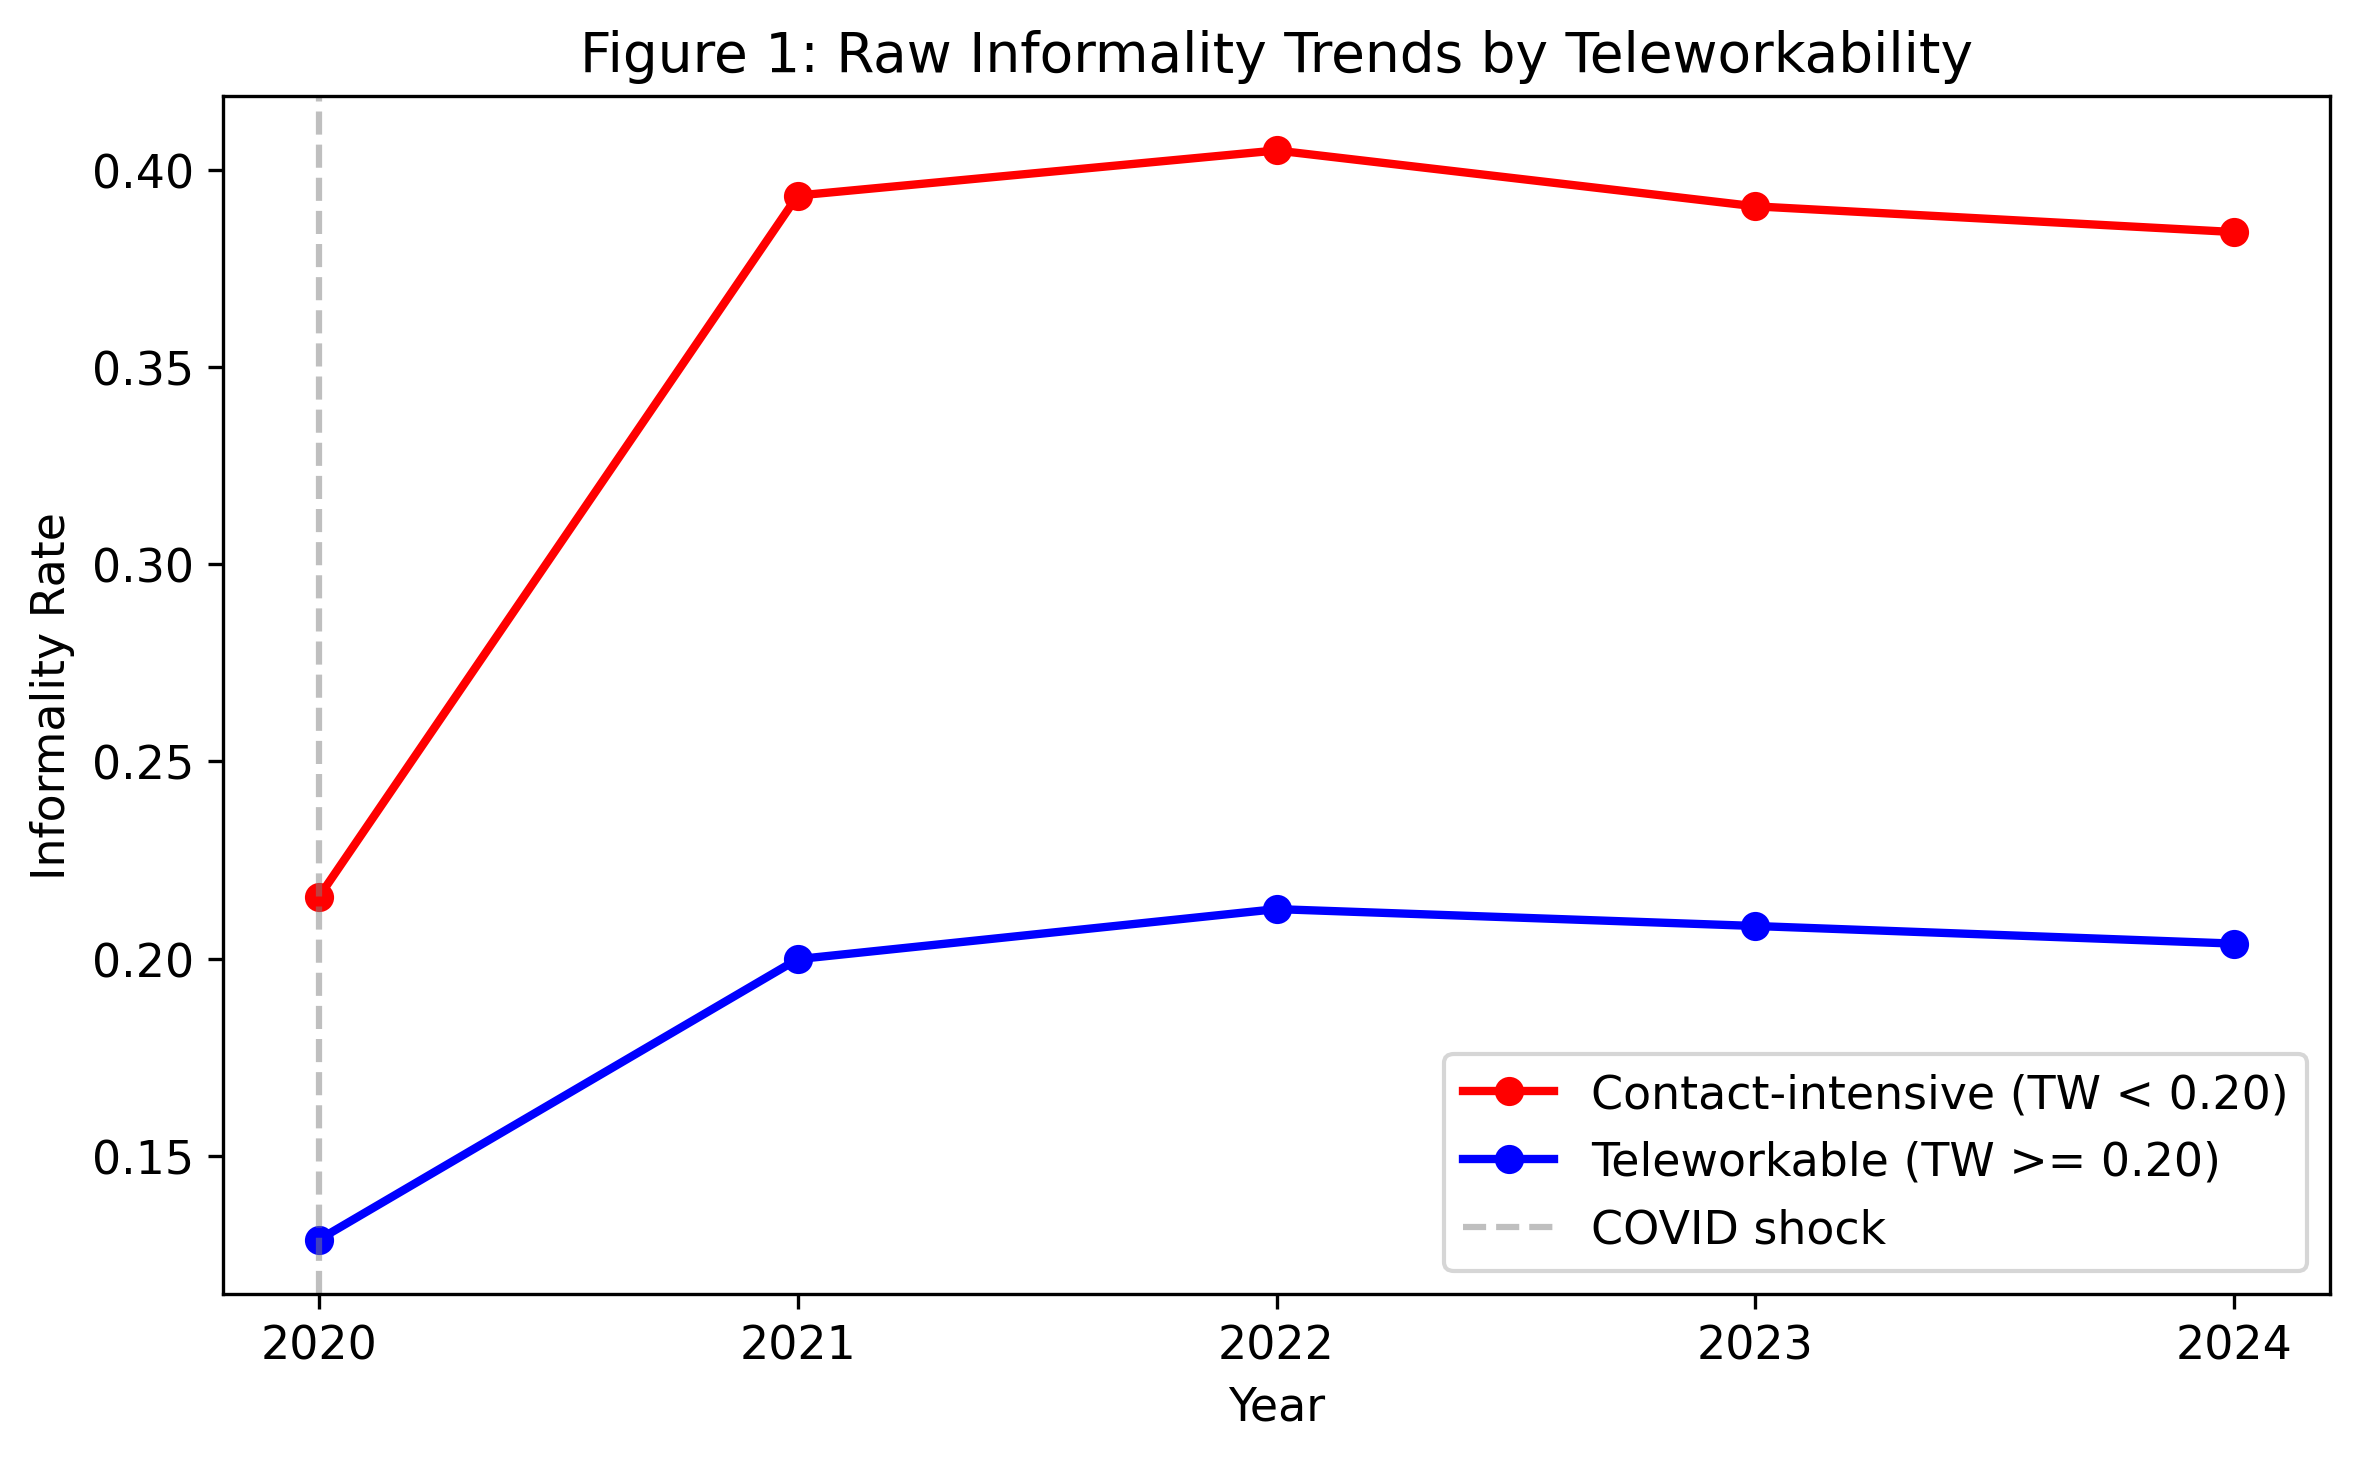
\includegraphics[width=\textwidth]{figures/fig1_raw_trends.png}
\caption{Raw Informality Trends by Teleworkability (2020--2024)}
\label{fig:raw_trends}
\end{figure}

\begin{figure}[H]
\centering
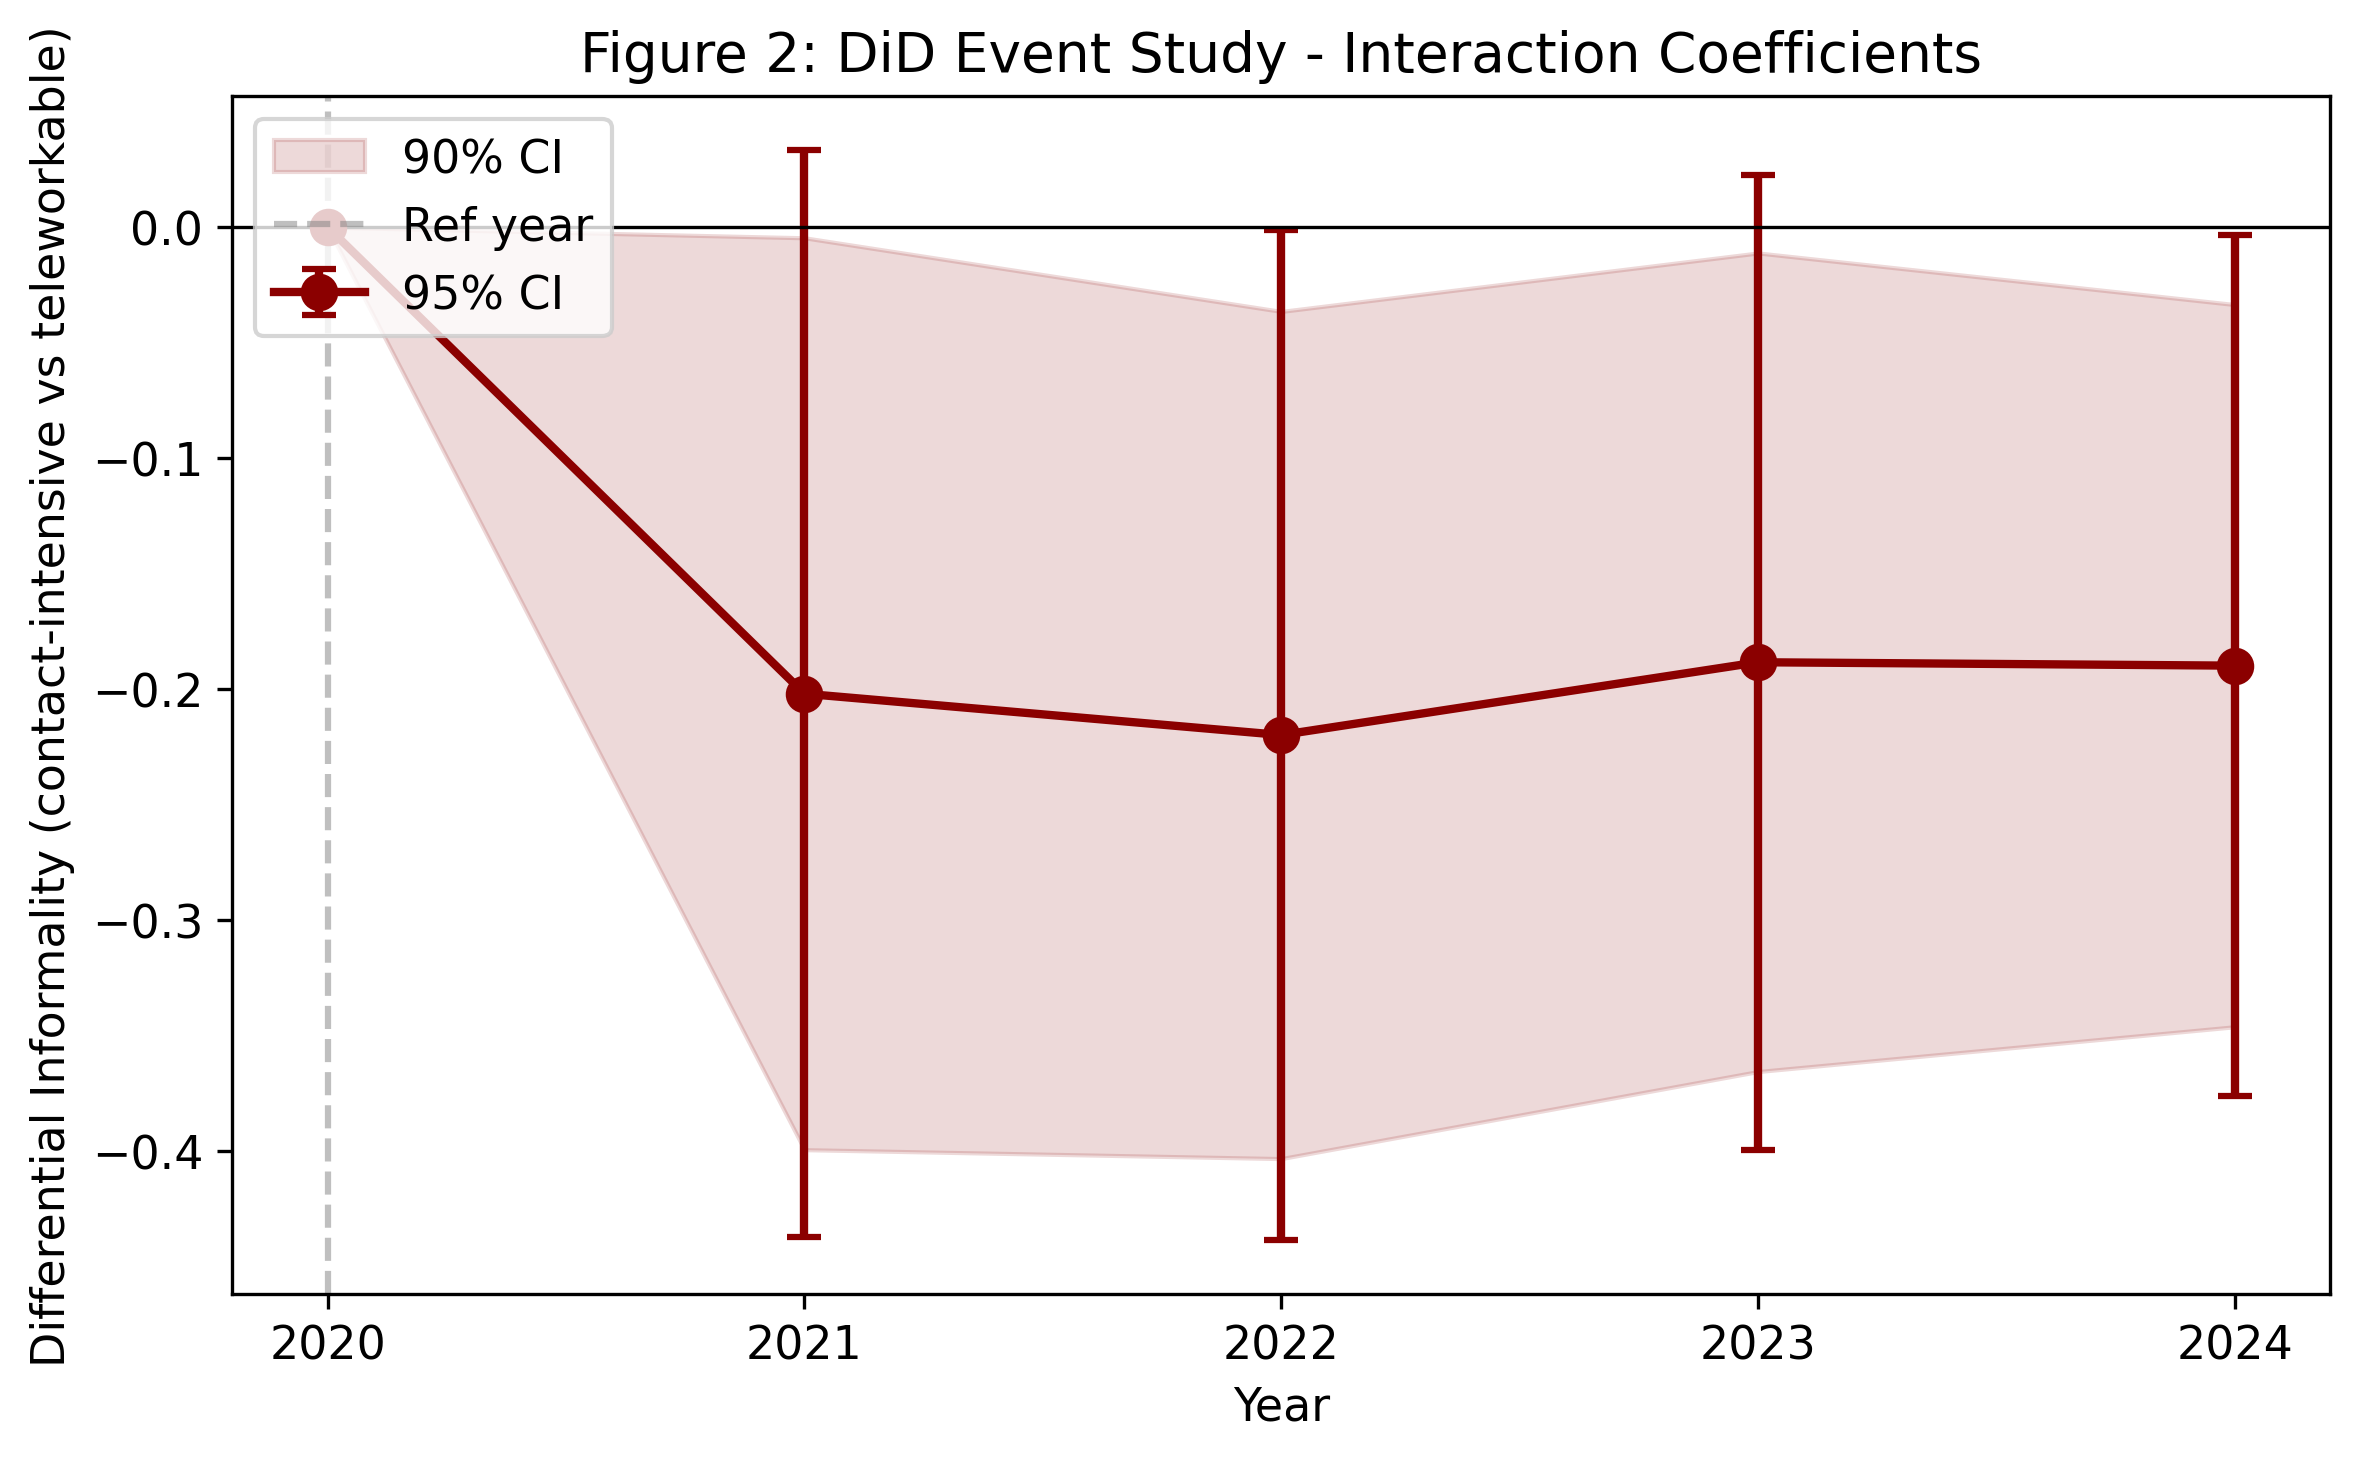
\includegraphics[width=0.85\textwidth]{figures/fig2_event_study.png}
\caption{DiD Event Study: Differential Informality for Contact-Intensive Workers}
\label{fig:event_study}
\end{figure}

\begin{figure}[H]
\centering
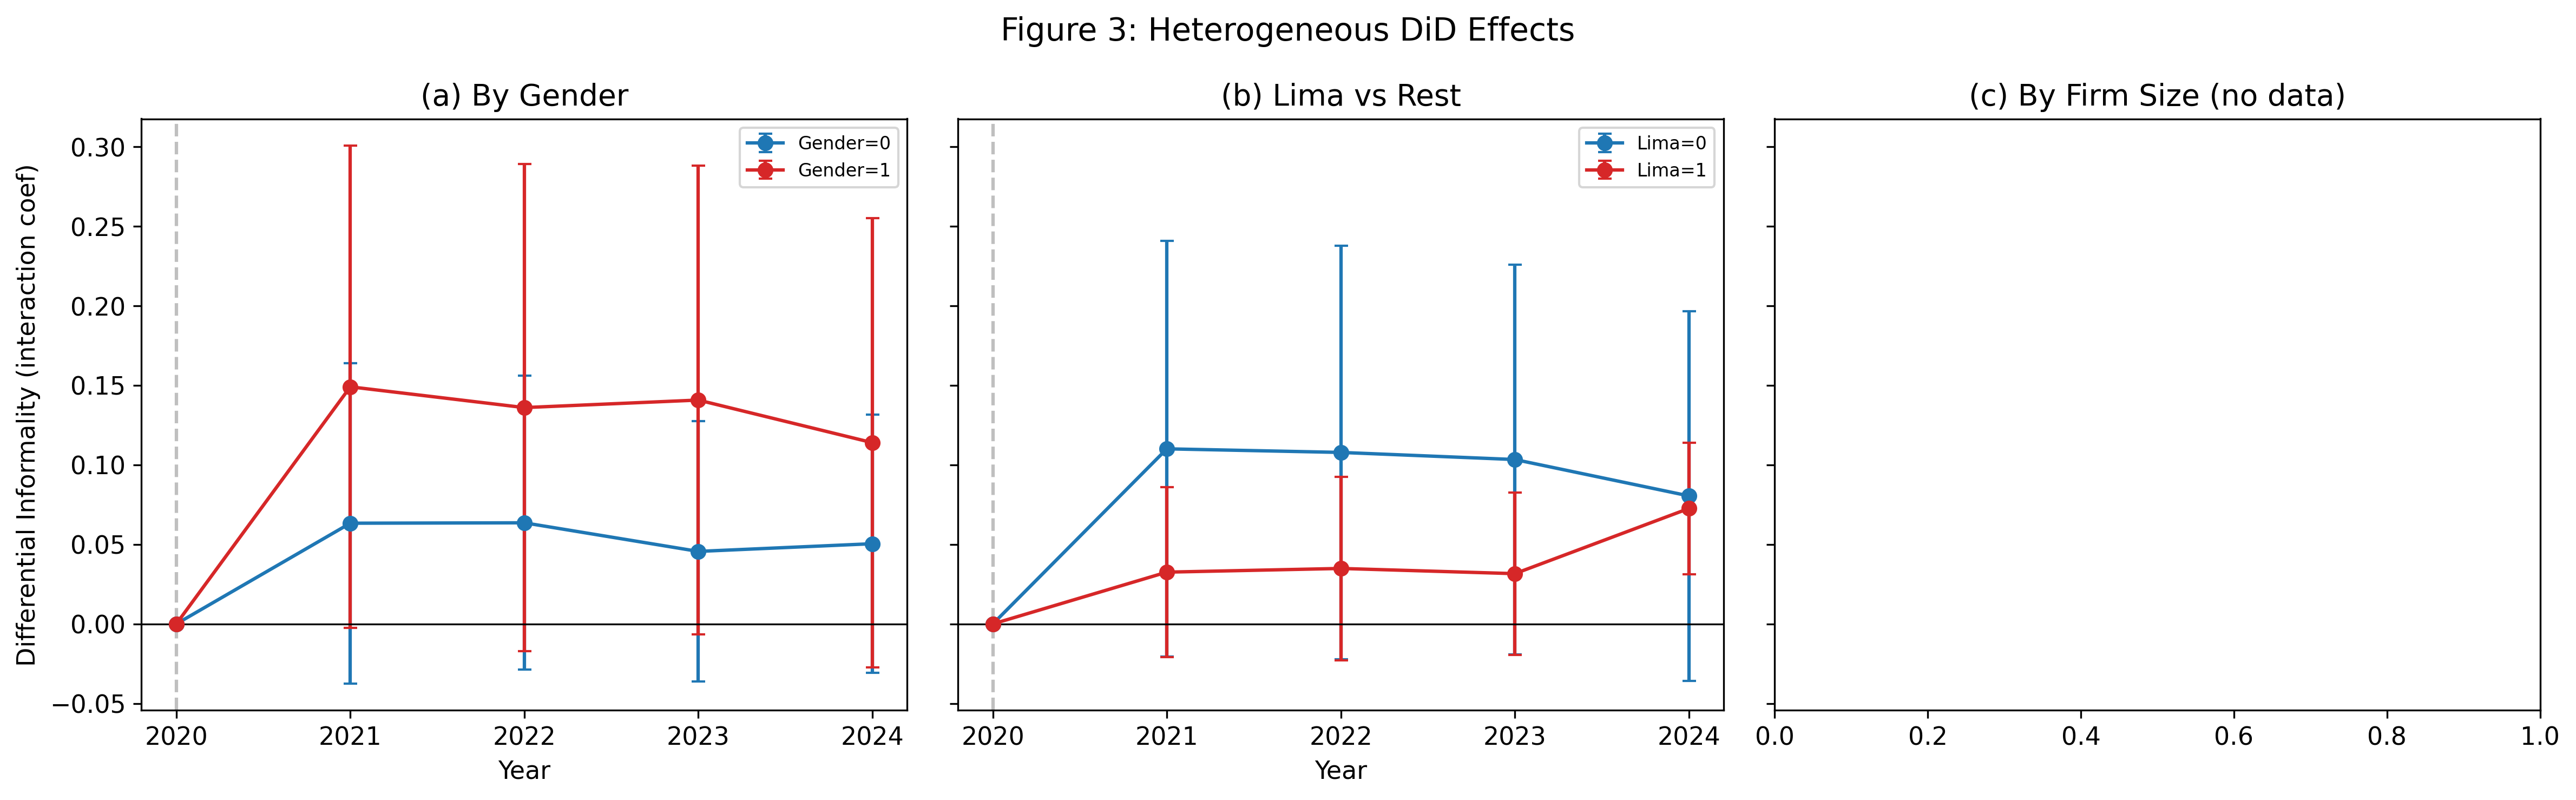
\includegraphics[width=\textwidth]{figures/fig3_heterogeneous.png}
\caption{Heterogeneous DiD Effects by Gender, Region, and Age Group}
\label{fig:heterogeneous}
\end{figure}

\clearpage
\bibliographystyle{apalike}
\bibliography{references}

\end{document}
